\documentclass{nature}
\bibliographystyle{naturemag}

\usepackage{amssymb}
\usepackage{graphicx}
\graphicspath{{figures/}}
\usepackage{lineno}
\linenumbers

% #magic #hack to make figures appear
\makeatletter
\let\saved@includegraphics\includegraphics
\AtBeginDocument{\let\includegraphics\saved@includegraphics}
\renewenvironment*{figure}{\@float{figure}}{\end@float}
\makeatother


\usepackage{color}

\usepackage[dvipsnames]{xcolor}

\definecolor{mygray}{gray}{0.6}


\newcommand{\todo}[1]{\textcolor{gray}{#1}}
\newcommand{\arxiv}{arXiv}

%\title{The differentiated impacts on academic productivity owing to the COVID-19 pandemic}
\title{The impact on academic productivity owing to the COVID-19 pandemic}

\author{Andrew R. Casey$^{\ast,1,2,}$,
        Ilya Mandel$^{\ast,1,2}$,
        Prasun K. Ray$^{3}$, 
        and friends?
}

\begin{document}

% Conclusions
% -> Most fields show no impact.
% -> Biggest negative impact is in fields where most research is presented at conferences, or experimental sub-fields.
% -> Condensed matter shows up-tick, where pre-prints have focussed on experimental design instead of experimental results.
% -> Biology has a peak, seems to be a lot of biologists posting to arxiv for the first time, or people contributing from other fields.

\maketitle

\begin{affiliations}
	\item School of Physics \& Astronomy, Monash University, Clayton 3800, Victoria, Australia
	\item Center of Excellence for Astrophysics in Three Dimensions (ASTRO-3D), Australia
	\item Department of Mathematics, Imperial College London, London, United Kingdom
\end{affiliations}

\begin{abstract}
	% Context.
	`\emph{Publish or perish}' is an expression that refers to the pressure on academics to consistently publish research to ensure a successful career in academia.
	% Define the gap, or question.
	With a global pandemic that has changed how businesses operate, has it also changed the academic publishing system?
	% Here we show.
%	Here we show that academics are collectively posting just as many publications as if there were no pandemic. 
%	This remains true across nearly all fields of research, including those focussed on theoretical and experimental research.
%	The most significant change in academic publishing is seen in biology, where there was a doubling of pre-prints posted in 2020. 
%	However, most of these extra pre-prints are not written by, or with, biologists.
%	\todo{At least half} of the excess biology pre-prints are entirely authored by researchers from other fields, primarily physicists.
%	No broad impact is found between theoretical and experimental research.
%	Reduced access to experimental laboratories seems to have motivated researchers to publish more papers (overall) based on work that was already in preparation. The full impact of the pandemic on academic publishing may not yet be fully realised.	
	Many fields undeterred; posting just as many as before.
	Some fields show a large increase (q-bio),
	Others, mostly experimental fields, show a marked decline in preprints.
	
\end{abstract}





%Some research fields have shown an explainable drop in research outputs due to the COVID-19 pandemic. Others have shown an increase, driven in part by shifts away from experimental research to topics that do not require ongoing access to laboratories. One thing in common between pre-prints 

%measure that is common among those fields where there is a change in pre-prints is the timescale: 



% Like many professions, in 2020 researchers worked remotely, in isolation, while balancing additional responsibilities like home-schooling children. Many academics rightfully report feeling their most unproductive. 

%Some sub-fields have already seen an explainable drop in research outputs due to the COVID-19 pandemic. For those fields without a measurable drop yet, it's plausible that either some academics are at their most productive while many are at their least, and it's plausible that many of the pre-prints being posted now are research projects that were well underway before the pandemic, with the full impact still to come.








%Part of this is due to name confusion, where two researchers in different fields share the same publishing name. However, a careful examination of pandemic-related pre-prints in quantitative biology posted in 2020 shows that many were posted by researchers from other fields (primarily physicists and mathematicians), who had never before posted about quantitative biology. 


% Here



% the field of quantitative biology peaked in 2020

%established 

% much of this increase in pre-prints was not written by a few 


%However,\todo{at least half} of these extra biology pre-prints were not written by established biologists. The number of new authors in quantitative biology peaked in 2020 (Figure~\ref{fig:new-authors-segmented-by-field}), while the number of new authors in all other fields remained steady. 



%However, these authors do appear in other \arxiv\ fields: in 2020 the author names in common between quantitative biology and other \arxiv\ fields spiked (Figure~\ref{fig:q-bio-pre-prints-with-author-overlap}). 
%These authors do appear in other \arxiv\ fields. In 2020 many of the pre-prints  in quantitative biology that are \emph{entirely} written by `new' authors (non-biologists) are authors that appear in other fields, primarily physicists and mathematicians. A careful cross-match of biology pre-prints with Google Scholar profiles shows that this statement is not conflated by two researchers with the same name that work in different fields. While it is possible that the COVID-19 pandemic inspired biologists to use \arxiv\ for the first time, this can only explain some of the excess biology pre-prints in 2020.





% -> How much? A doubling
% -> Driven entirely by COVID-papers.
% -> Author make-up.



% -> People wrote papers about COVID in other fields.



%Pre-prints in lattice physics (hep-lat) periodically peak around December each year as conference proceedings from the International Symposium on Lattice Field Theory are posted to \arxiv. In 2020 the conference was cancelled, so no accompanying pre-prints exist. The impact on research from travel restrictions and cancelled conferences is likely to be much longer term than what is represented by the drop in lattice physics pre-prints.   Conference discussions or collaborative visits frequently spark new research ideas that might lead to a publication many months later. Some research ideas require laboratories or specialised equipment to be built, or data to be collected over years. Depending on the research, a single publication may represent the work of weeks, years, or even a decade. 



%In some fields there are significant deviations from the model predictions, indicative of the differentiated impact the COVID-19 pandemic has had on academic productivity. The most significant deviation is in quantitative biology (\arxiv\ code `q-bio'), where 2020 saw about double the number of pre-prints than expected (\todo{$X^{X}_{X}$} expected, \todo{$Y$} observed). The titles and abstracts of these pre-prints shows that the excess biology pre-prints is entirely due to research related to the SARS-CoV-2 disease or the COVID-19 pandemic (Figure~\ref{fig:pandemic-related-preprints}). In March 2020, nearly 60\% of pre-prints in quantitative biology were related to the COVID-19 pandemic.


%, with most pre-prints appearing in the sub-field of \emph{Populations and Evolution} (q-bio.PE; Figure~\ref{fig:q-bio-pre-prints-with-entirely-new-authors}).


%An increase in biology research during a global pandemic is not surprising. However,\todo{at least half} of these extra biology pre-prints were not written by established biologists. The number of new authors in quantitative biology peaked in 2020 (Figure~\ref{fig:new-authors-segmented-by-field}), while the number of new authors in all other fields remained steady. The sudden influx of new authors cannot be explained by large newly-formed collaborations working together to tackle the impending pandemic (Figure~\ref{fig:q-bio-pre-prints-segmented-by-author-count}).  The increase in pre-prints (and new authors) is driven by small (1-4) groups of authors who had never before posted pre-prints to biology before, either as leading- or co-author (Figure~\ref{fig:pre-prints-with-entirely-new-authors}). 
%However, these authors do appear in other \arxiv\ fields: in 2020 the author names in common between quantitative biology and other \arxiv\ fields spiked (Figure~\ref{fig:q-bio-pre-prints-with-author-overlap}). 
%These authors do appear in other \arxiv\ fields. In 2020 many of the pre-prints  in quantitative biology that are \emph{entirely} written by `new' authors (non-biologists) are authors that appear in other fields, primarily physicists and mathematicians. A careful cross-match of biology pre-prints with Google Scholar profiles shows that this statement is not conflated by two researchers with the same name that work in different fields. While it is possible that the COVID-19 pandemic inspired biologists to use \arxiv\ for the first time, this can only explain some of the excess biology pre-prints in 2020.
 

%While some biologists continued to post to \arxiv\ for the first time in 2020, the sharp increase in biology pre-prints in 2020 is driven by researchers from other fields.

%Physicists and mathematicians devoting time to research topics related to COVID-19  could be good or bad. Here we are reporting only on the quantity of pre-prints, which has no bearing on their quality or impact. Many COVID-19 pre-prints posted in 2020 by physicists and mathematicians have no expert biologist as a co-author. Is it still considered multi-disciplinary research -- a research trait fertilised by many institutions worldwide -- to publish in another field without any subject domain experts? Are academics spending time trying to advance efforts against the most significant problem to face society this year, or are some jumping on a citation-laden bandwagon? The impact of these pre-prints is hard to measure. The number of citations are routinely used as a measure of research impact, but that metric becomes less useful in a period where pre-prints are being written (and cross-citing each other) faster than those pre-prints are being read.

%in 2020 the author names in common between quantitative biology and other \arxiv\ fields spiked 

% rlap in common names between different fields spiked well above the pre-pandemic 


%We examined the number of pre-prints posted in \emph{Populations and Evolution} (q-bio.PE) where those author names had never appeared in any quantitative biology (q-bio) field before, but those names do appear in other \arxiv\ fields .

% This gives a measure of the number of common names between different fields before the pandemic, which is about 1-3\%. In 2020 most of the pre-prints in 
%The fields with the largest number of unique names are, in order: computer science, physics, condensed matter, math, and astrophysics. While it is more likely to have names overlapping between biology and computer science (the largest field by unique names) by chance, the newly authored pre-prints in quantitative biology in 2020 are driven by physicists and mathematicians. 
%Taking the number of pre-prints in \emph{Populations and Evolution} (q-bio.PE) where no author has appeared before in that sub-field, at least 40\% of these pre-prints are written by researchers from other fields. 



%With physicists and mathematicians seemingly having time to write research papers in quantitative biology, one might expect a corresponding drop in physics or math pre-prints. No drop is evident in maths. Physics showed no average drop over the year, but this is balanced by an uncharacteristic increase in pre-prints in the first half of 2020 (the same time the quantitative biology peak occurred), and a drop in the second half. However, some sub-fields of experimental physics were noticeably impacted by COVID-19. 
%Even limiting access to compute facilities may have had a substantial effect on theoretical research. 
%The field of computational physics (physics.comp-ph) saw a severe decline in research outputs from June 2020, reducing pre-prints to a level not seen in five years. If this drop is a causal effect of the pandemic, it is the strongest relative decline seen in any sub-field. 
%High energy experimental physics pre-prints dropped sharply in January 2020 ($\sim$20\% compared to 2019 levels), and remained low throughout 2020, likely due in part to limited laboratory access. Access to laboratories is also critical for condensed matter research, but this field saw a slight increase in total pre-prints, in part driven by a 20\% increase in material science pre-prints (cond-mat.mtrl-sci), a sub-field of condensed matter that focusses on laboratory methods and techniques. Without access to laboratories, this increase may be a consequence of `writing up what we can': a motivation to publish existing work that would otherwise be neglected due to ongoing laboratory work.








%While the number of pre-prints within primary research fields has remained largely unchanged during the pandemic, there have been noticeable changes within specific sub-fields. Border restrictions have obviously limited field work and the capacity to attend conferences. In the field of high energy physics (lattice), pre-prints tend to peak around December each year as research presented at the International Symposium on Lattice Field Theory conference is posted on \arxiv. In 2020 no Lattice Field Theory conference was held\footnote{The last Lattice Field Theory conference was coincidentally held in Wuhan, Hubei, China.}, so no accompanying pre-prints were posted (Figure~\ref{fig:new-authors-segmented-by-field}). 




% Within the field of computational physics (physics.comp-ph) the first half of 2020 saw a slight increase in pre-prints that was consistent with the rise in recent years. By June 2020 that peak began to fall, and continued to do so until the extent of the data (January 2021), where new pre-prints were at the lowest level seen in about five years. If this drop is a causal effect of the pandemic, it is the strongest relative decline seen in any sub-field.






%We hypothesise that this is in part attributed to the long timescales of academic research, and (as we discuss below) the differentiated impact the COVID-19 pandemic has had. Collectively academics may have published just as many research papers, but this may be driven by some individuals writing more papers, and many individuals writing fewer.






%Depending on the research, a single publication may represent the work of months or years. Conference discussions or collaborative visits frequently spark new research ideas that lead to publication a year or more later. With travel restrictions introduced early- to mid-2020, any decline in preprints may not be visible in a field for some time.



%Experimental physics fields either showed a drop in total preprint counts, or a shift towards writing methods-based publications that no longer require laboratory access. 


%Usually these techniques are developed as part of an ongoing experiment, and then published separately once the primary (`more interesting') research is complete. 

% However, there were no accompanying sharp declines in any other categories of materials science: overall there were more publications across all fields of condensed matter, not fewer.




%The impact of reduced travel is most clearly seen in high energy lattice physics preprints, where a yearly conference is held each year and research is presented. Instead of running this conference virtually, in 2020 it was cancelled, and no associated pre-prints were posted.

%The field of high energy physics saw an almost immediate reduction of about 20\% fewer pre-prints posted per month, a drop that persisted throughout 2020.






% Many research projects take months or years to complete. It is reasonable to suspect that the full effect of the pandemic has yet to be realised on pre-print counts, while academics publish what they can within ongoing restrictions.


% because full impact not known yet

%hep ex
%physics
%q-fin
% biology stsuff







%While the number of pre-prints within primary research fields has remained largely unchanged during the pandemic, there have been noticeable changes within specific sub-fields. Border restrictions have obviously limited field work and the capacity to attend conferences. In the field of high energy physics (lattice), pre-prints tend to peak around December each year as research presented at the International Symposium on Lattice Field Theory conference is posted on \arxiv. In 2020 no Lattice Field Theory conference was held\footnote{The last Lattice Field Theory conference was coincidentally held in Wuhan, Hubei, China.}, so no accompanying pre-prints were posted (Figure~\ref{fig:new-authors-segmented-by-field}). 


%\noindent\todo{physics.soc-ph saw a bump due to COVID-related research}


 \begin{figure}
 	\centering
     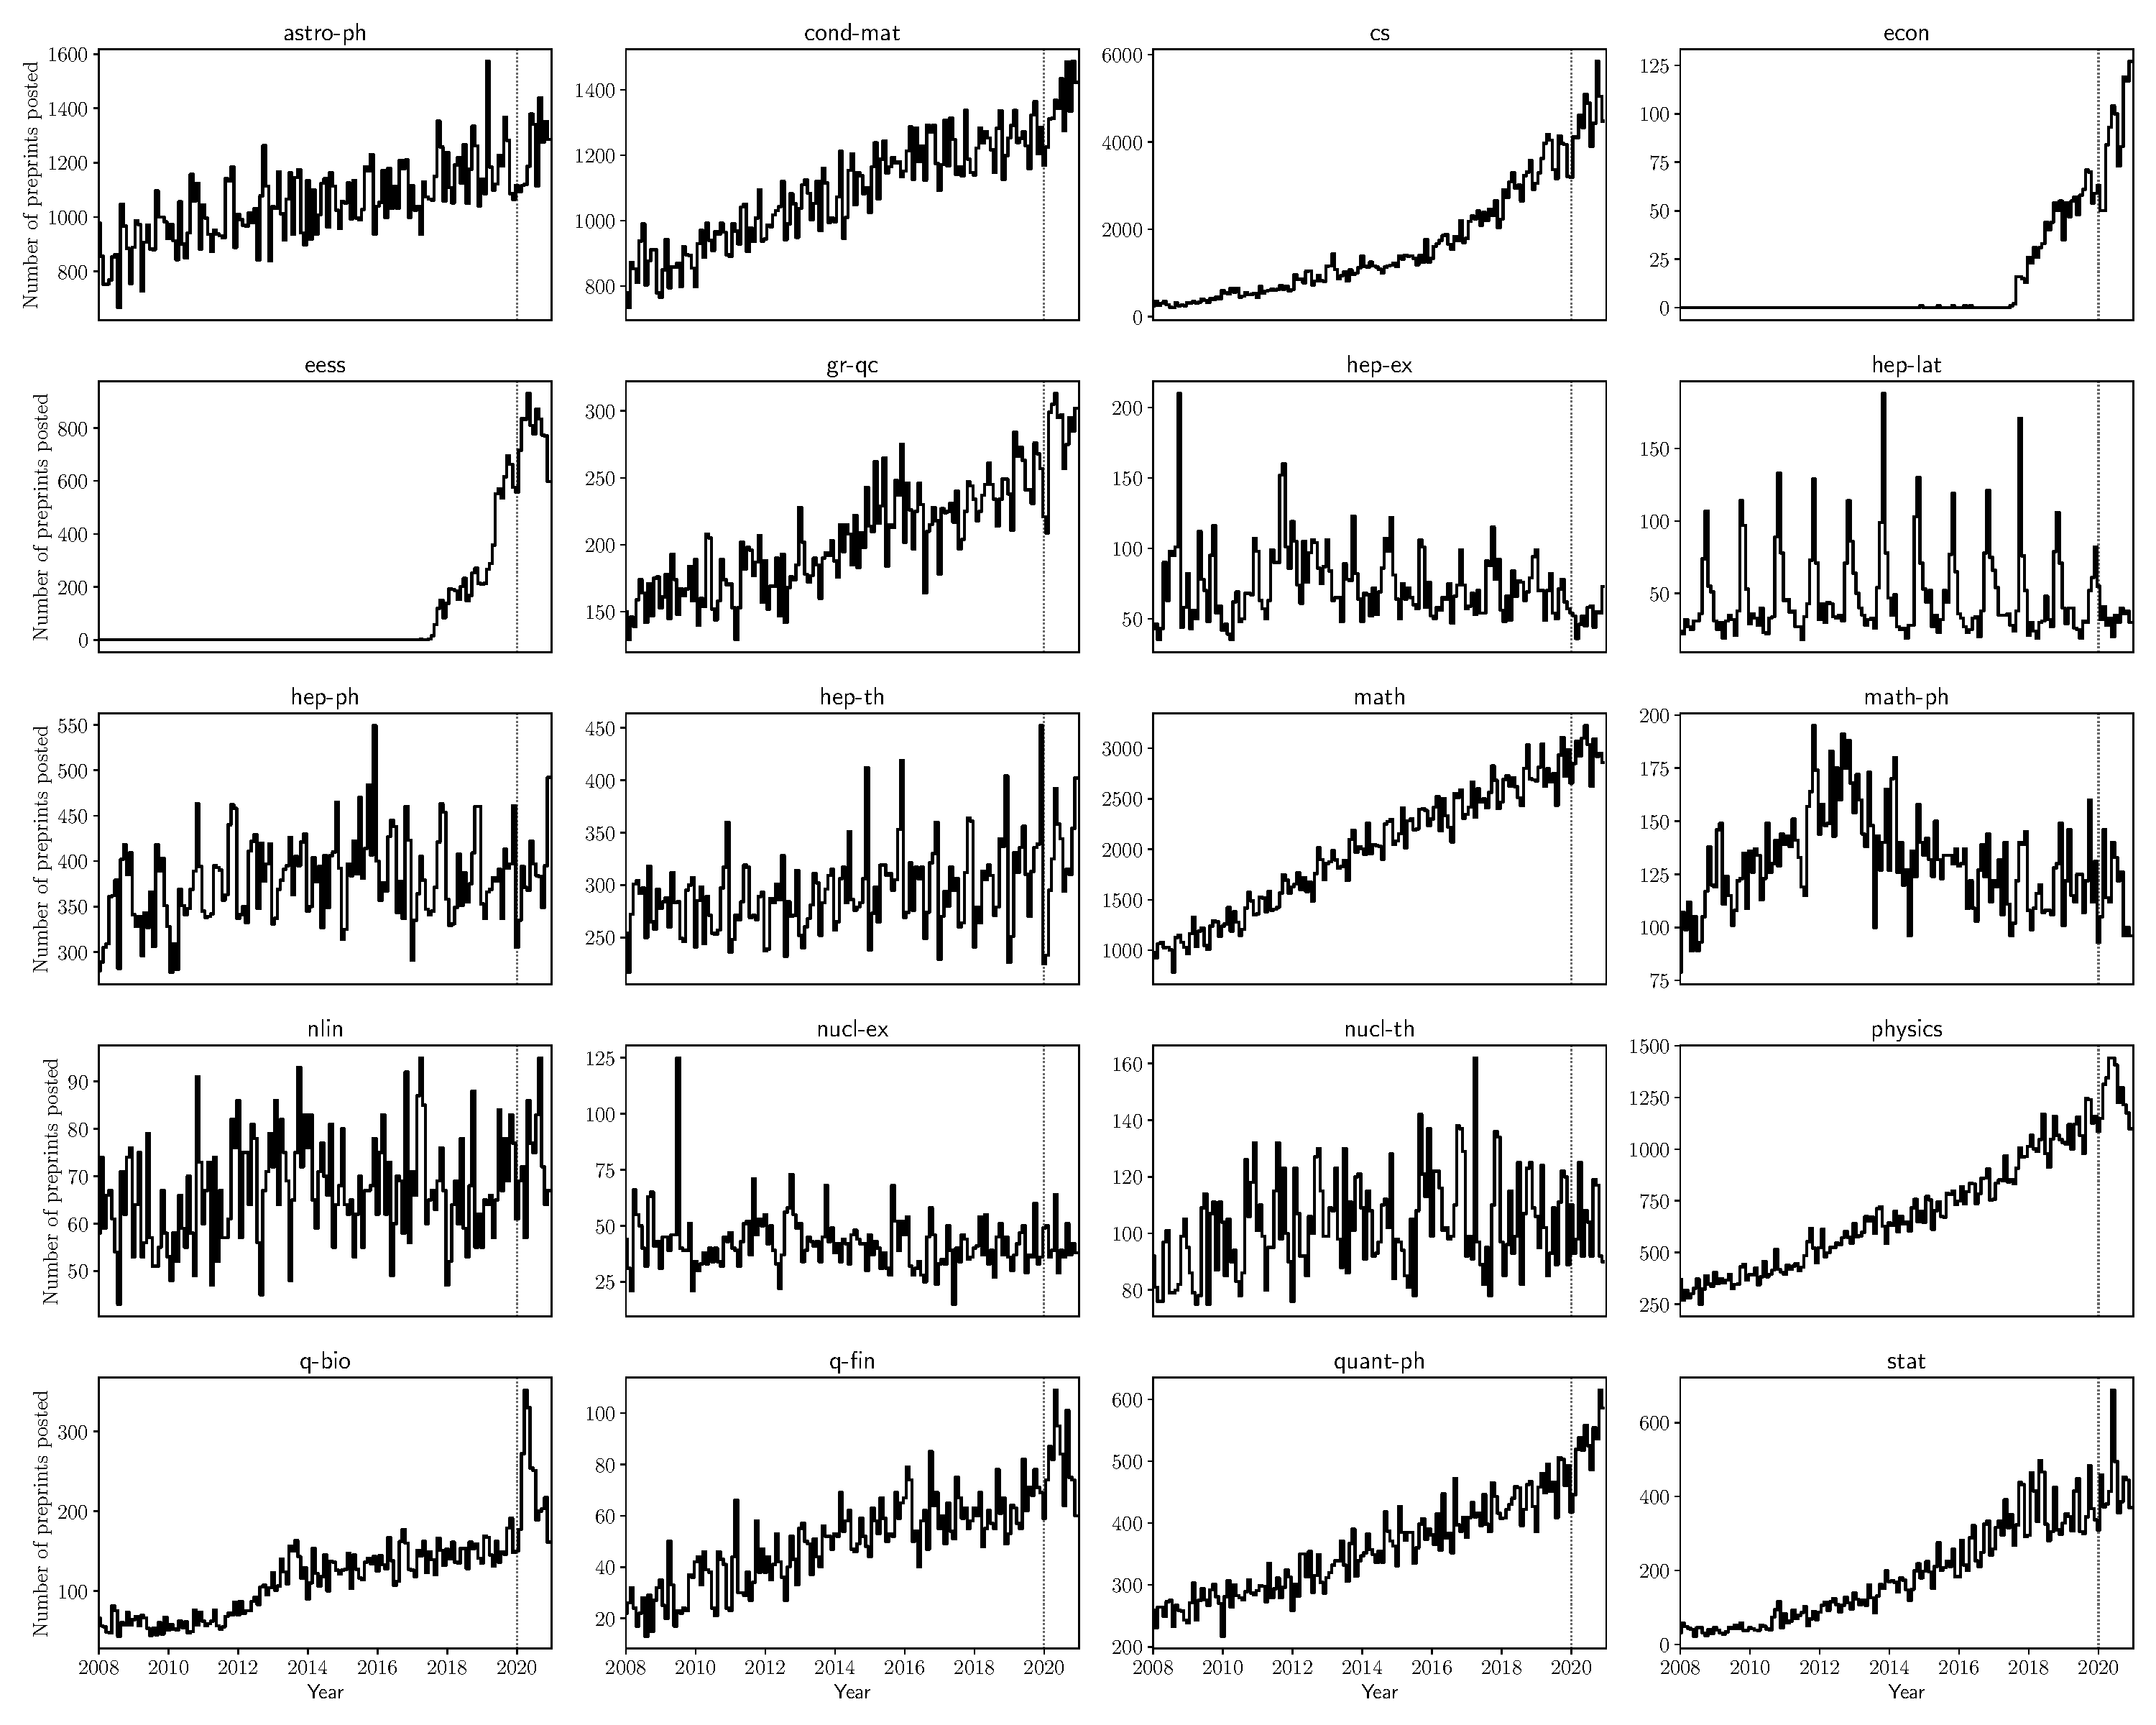
\includegraphics[width=0.95\textwidth]{pre-prints-segmented-by-field}
     \caption{Most fields saw no change in the number of pre-prints posted due to the COVID-19 pandemic. \todo{The model.} The exception is quantitative biology (q-bio), where the spike in 2020 is in part caused by COVID-19 related pre-prints authored by people who are non-established biologists.}
     \label{fig:pre-prints-segmented-by-field}
 \end{figure}
 
%\begin{figure}
%	\centering
%	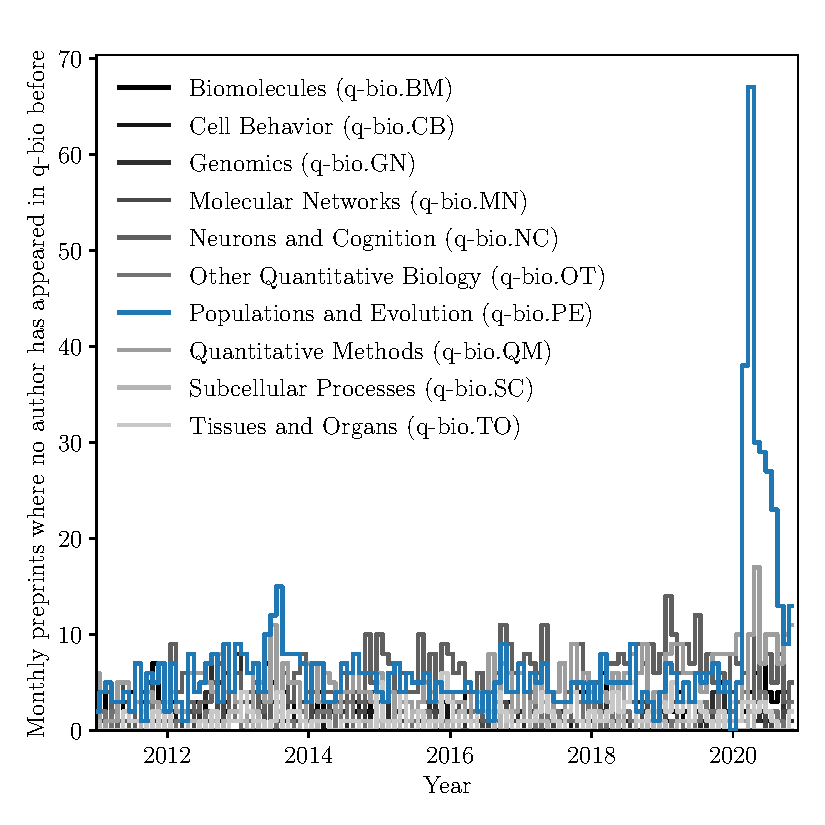
\includegraphics[width=0.65\textwidth]{q-bio-pre-prints-with-entirely-new-authors}
%	\caption{In 2020 there was a sharp increase in \emph{Populations and Evolution} (q-bio.PE; blue) pre-prints that were seemingly written without a biologist.  Here we show the number of \arxiv\ pre-prints posted per month where \emph{no author} had ever before appeared on a biology pre-print before, grouped by the primary category. The number of pre-prints per category remains stable with time, except for \emph{Populations and Evolution} (q-bio.PE) in 2020, which saw an influx of pre-prints where no author had ever appeared on a biology pre-print before.}
%	\label{fig:q-bio-pre-prints-with-entirely-new-authors}
%\end{figure}

\begin{figure}
	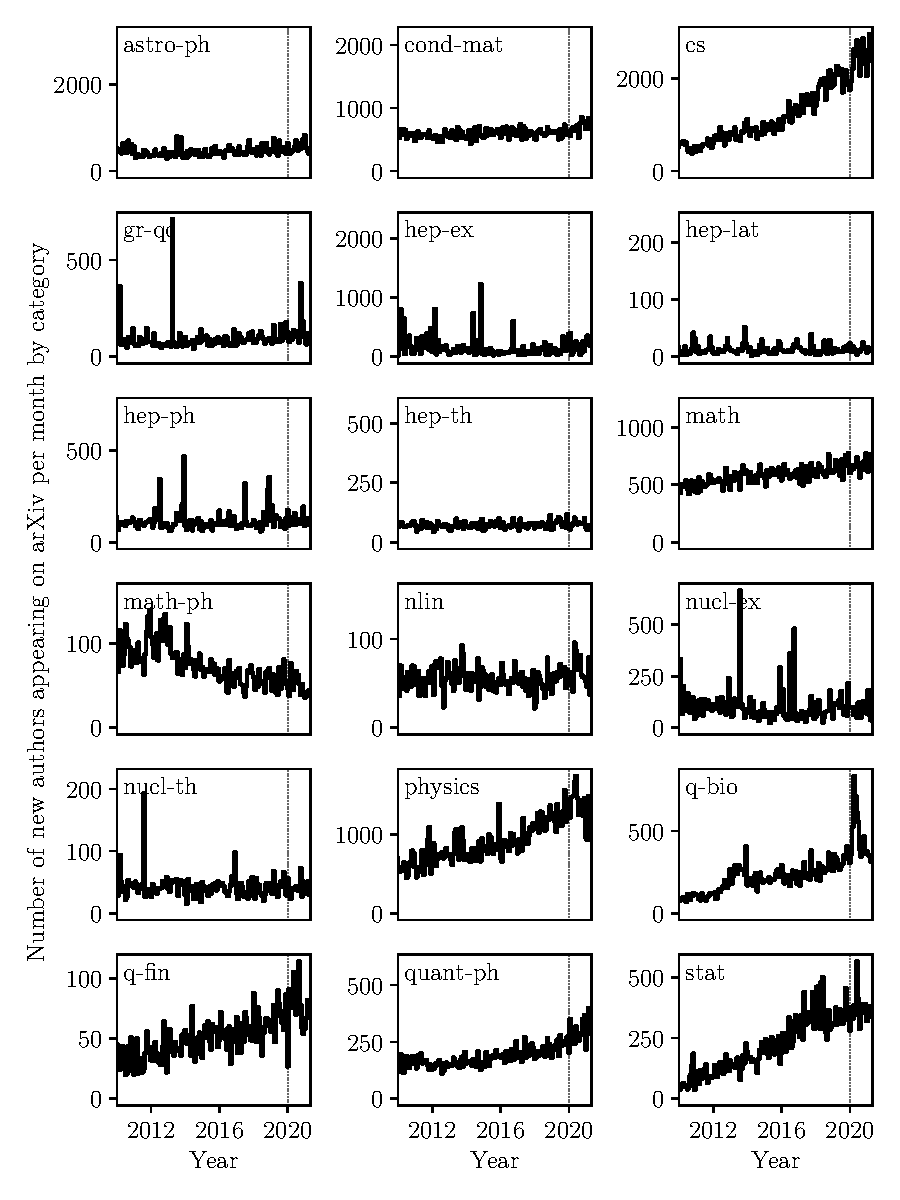
\includegraphics[width=\textwidth]{new-authors-segmented-by-field}
	\caption{The number of new author names appearing in the literature by field. Fields established well before 2007 (e.g., astro-ph) show an apparent influx of authors at the time the data starts (2007). These author names are dominated by established academics. The slow change in new author count after 2010 approximates the net number of new academics joining the field. Note the spike in new authors in quantitative biology in 2020.}
		\label{fig:new-authors-segmented-by-field}
\end{figure}

  \begin{figure}
  	\centering
     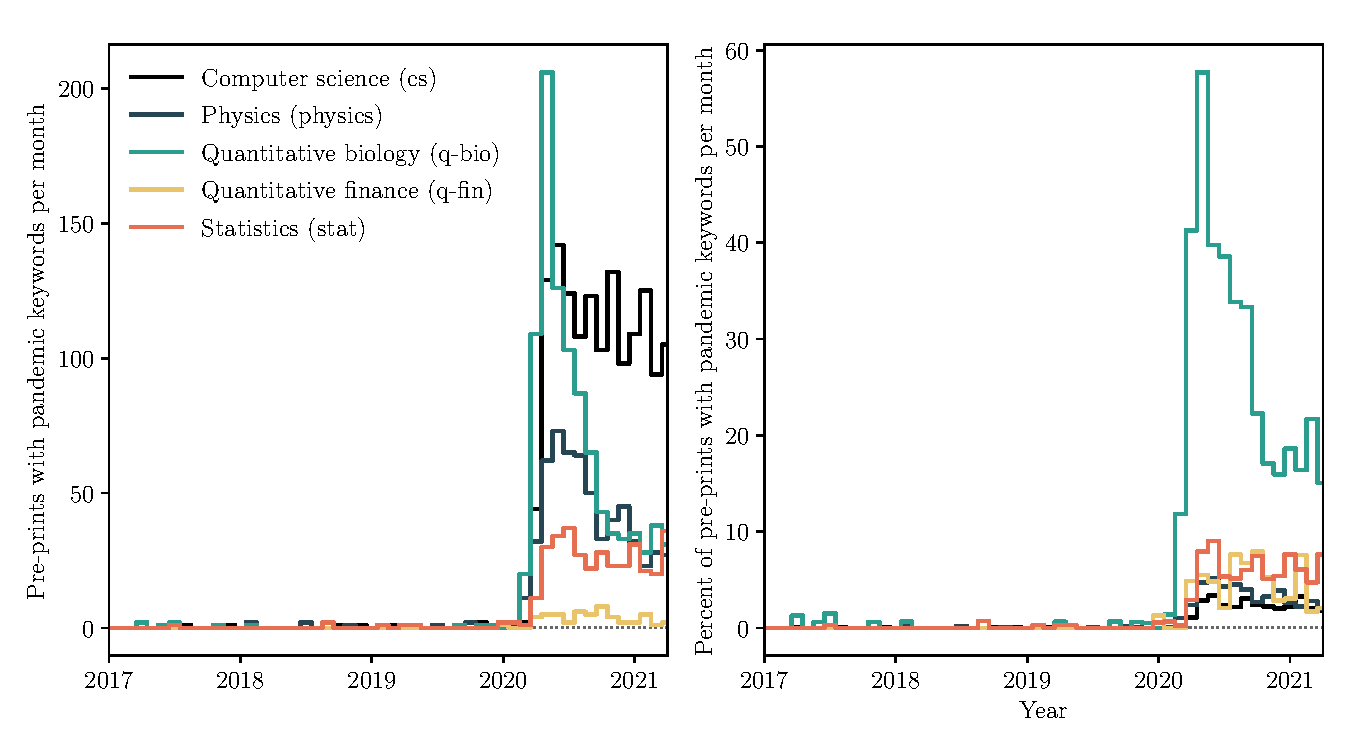
\includegraphics[width=\textwidth]{pandemic-related-preprints.pdf}
     \caption{}
     \label{fig:pandemic-related-preprints}
       \end{figure}

 
  \begin{figure}
  	\centering
     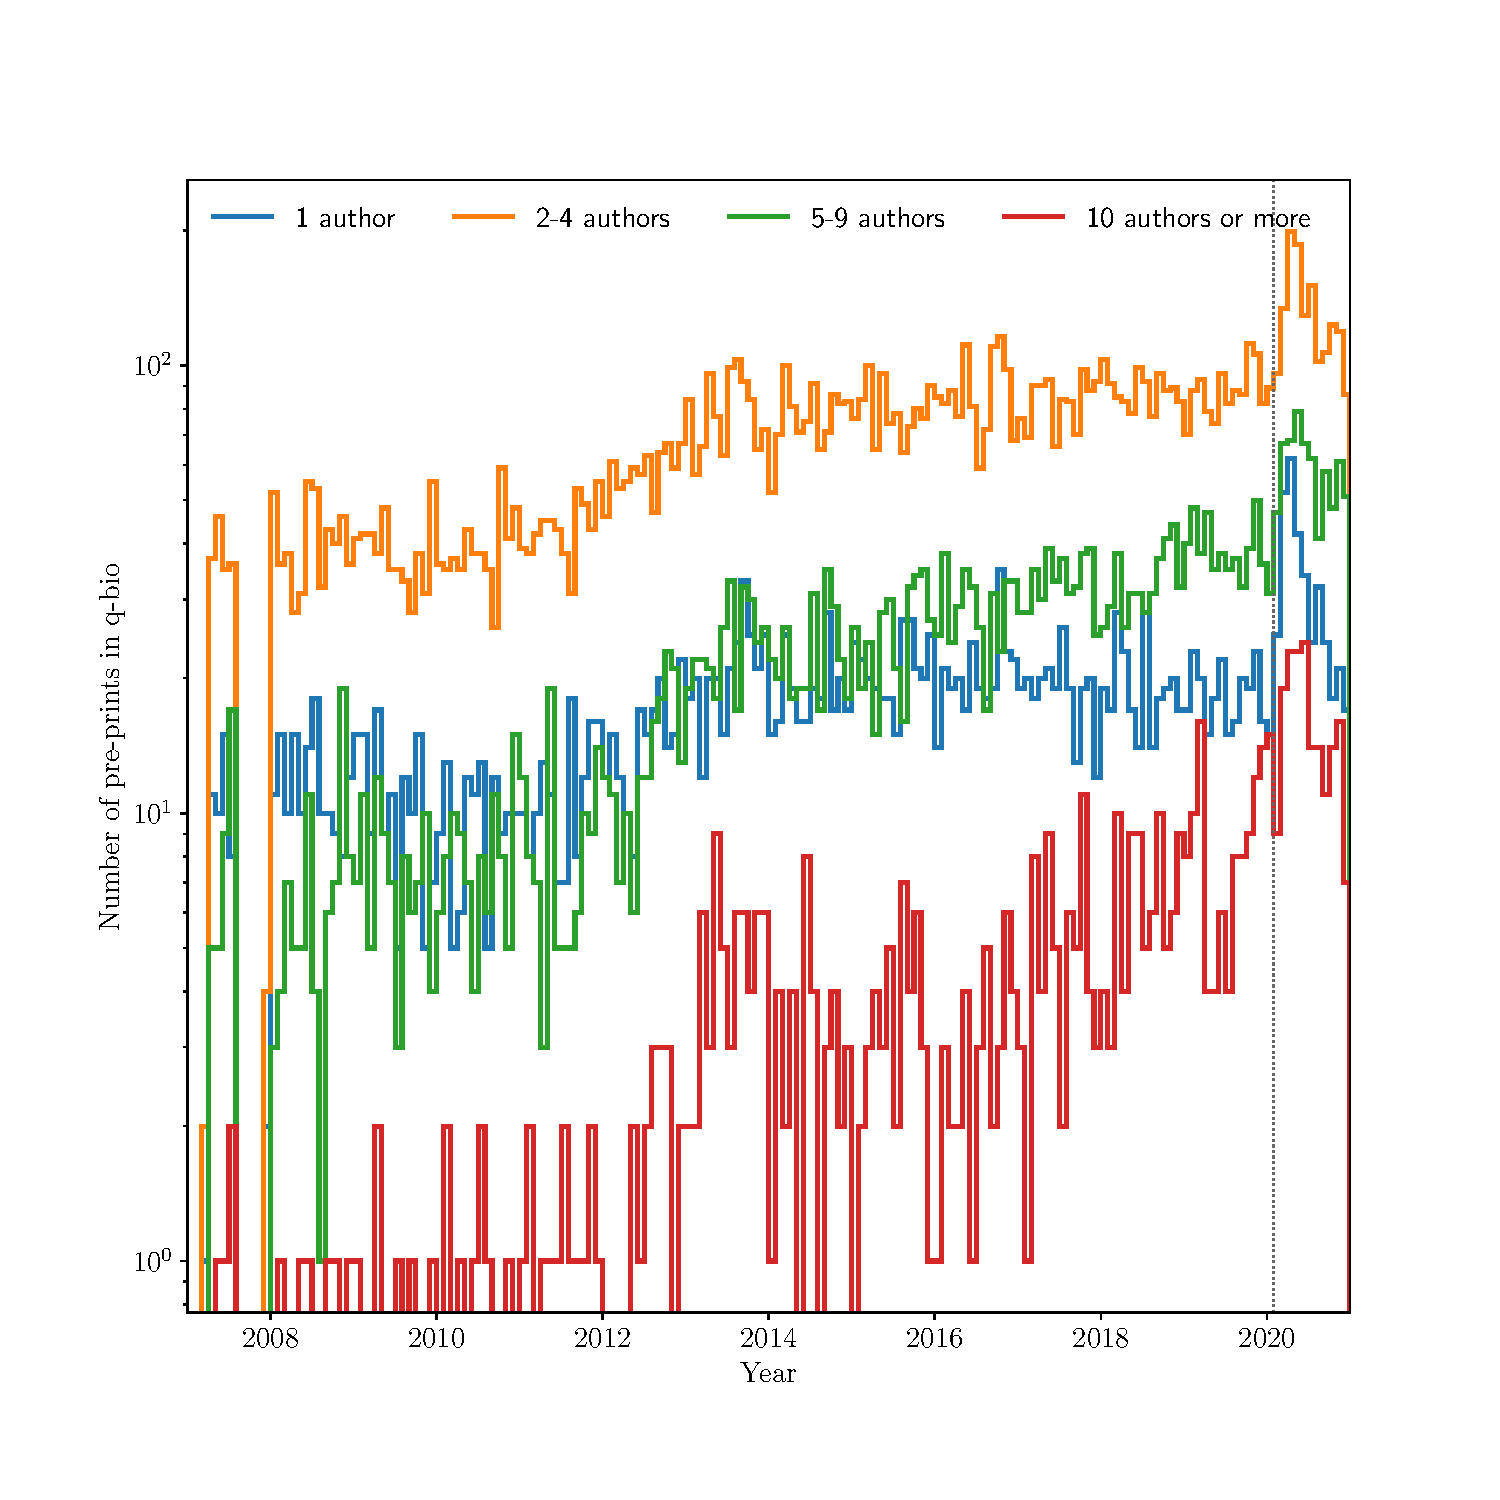
\includegraphics[width=0.5\textwidth]{q-bio-pre-prints-segmented-by-author-count}
     \caption{The increase in quantitative biology pre-prints in 2020 cannot be attributed to large collaborations. Here we segment q-bio pre-prints by the number of authors, showing that in 2020 a sharp increase was observed for single-author papers and small (2-4 authors) collaborations.}
     \label{fig:q-bio-pre-prints-segmented-by-author-count}
  \end{figure}

% ARC: no longer needed as covered by Figure 2
%\begin{figure}
%	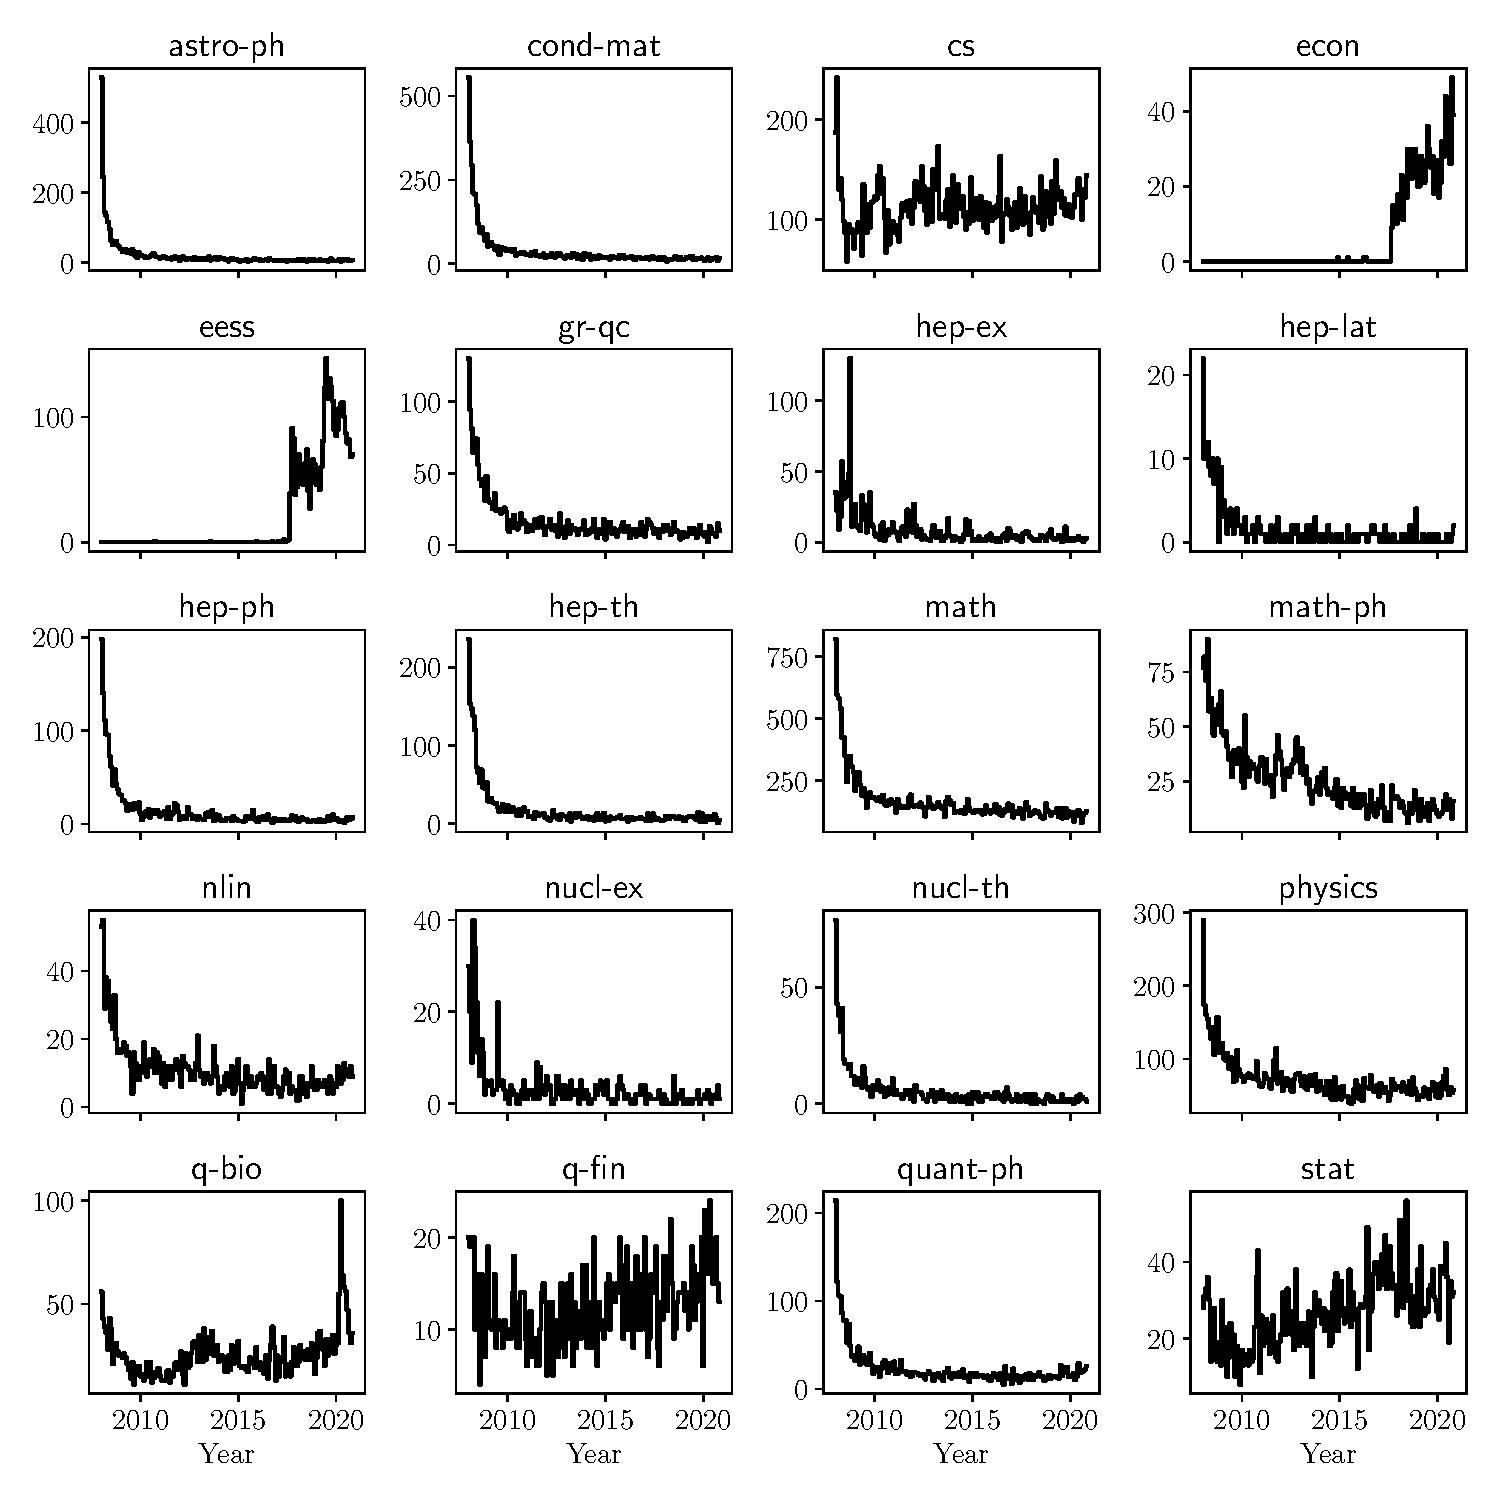
\includegraphics[width=\textwidth]{pre-prints-with-entirely-new-authors}
%	\caption{The number of pre-prints appearing per field where all authors have never appeared in the literature for that field before. A sharp increase remains present for quantitative biology (q-bio), representing an influx of pre-prints entirely written by authors who had never posted to \arxiv/q-bio before.}
%		\label{fig:pre-prints-with-entirely-new-authors}
%\end{figure}


%  \begin{figure}
%     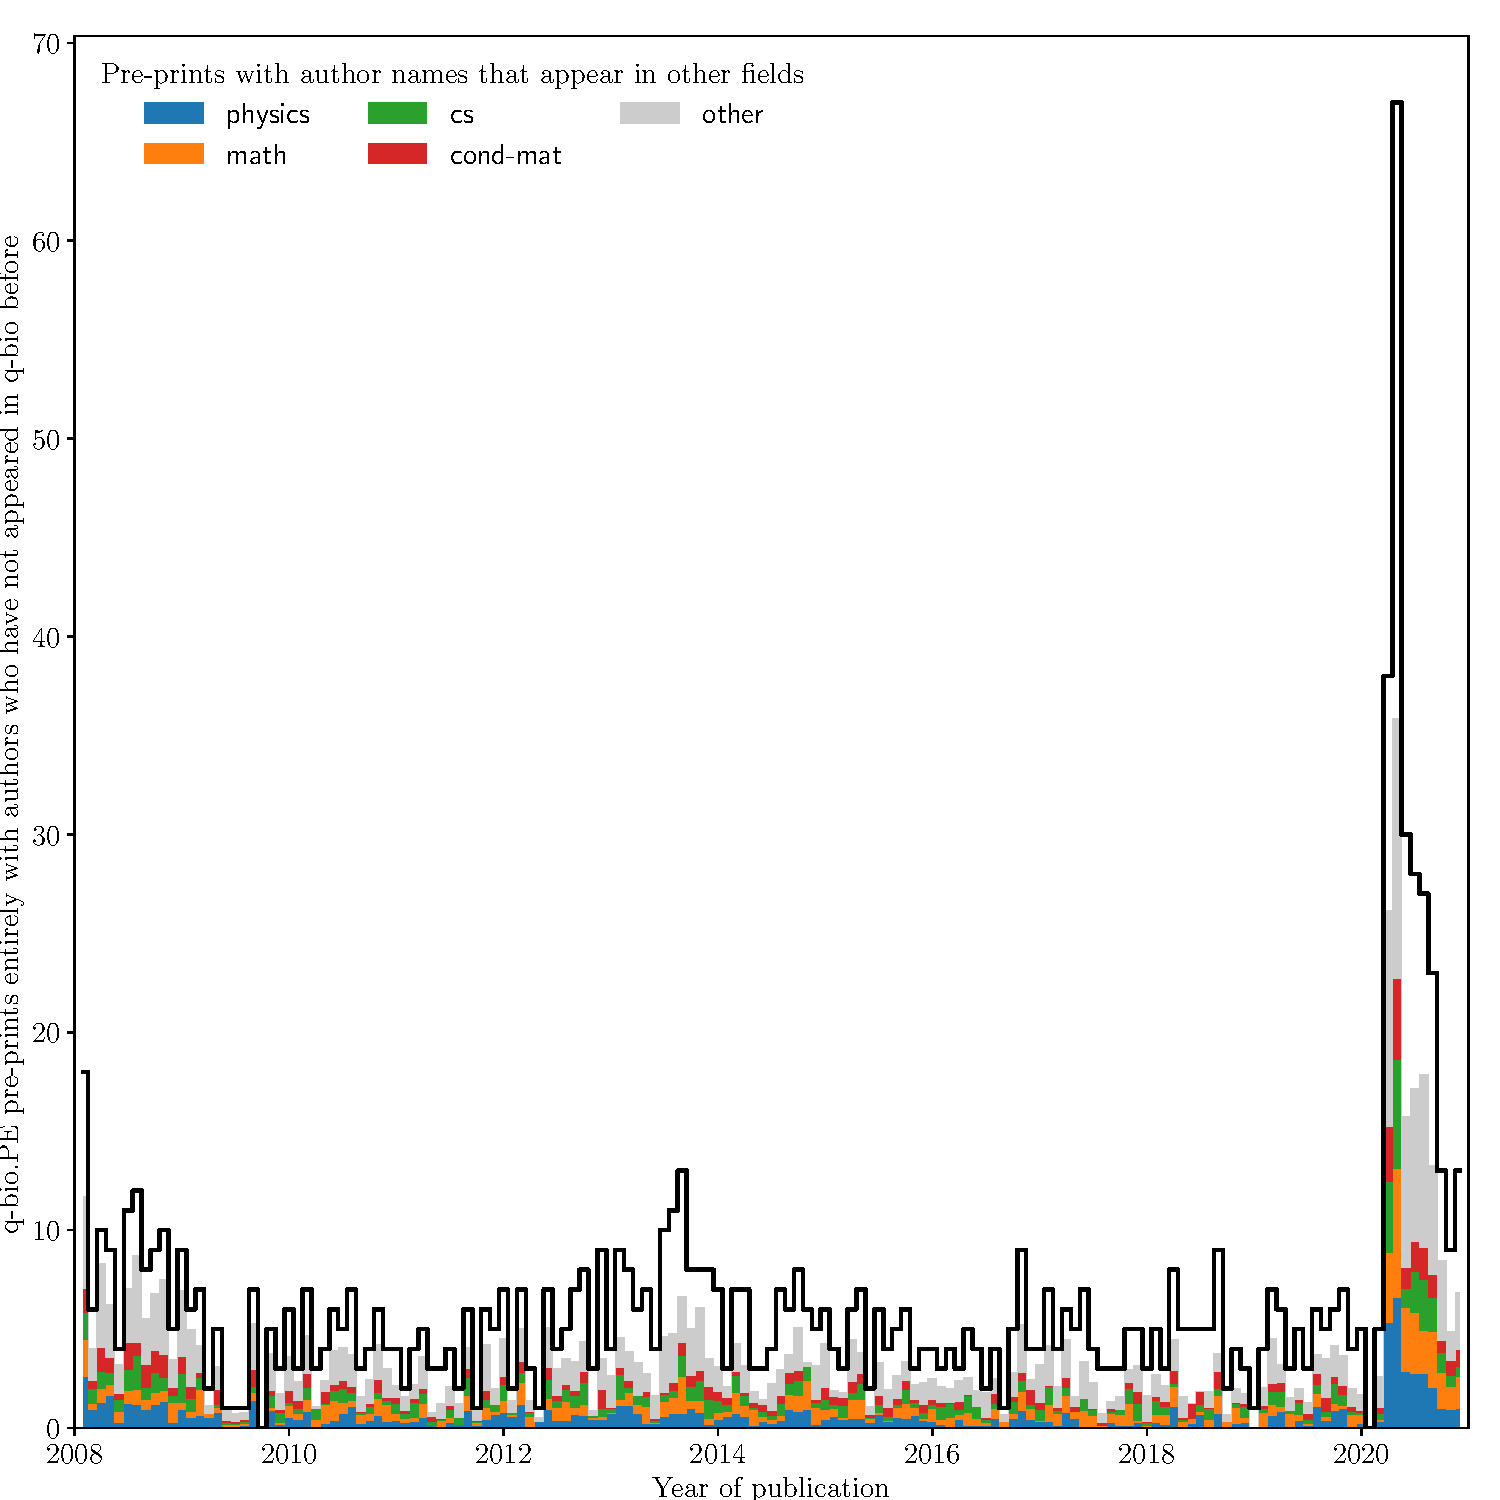
\includegraphics[width=\textwidth]{q-bio-pre-prints-with-author-overlap}
%%     \caption{Many physicists and mathematicians posted pre-prints to quantitative biology in 2020 for the first time. Pre-prints in \emph{Populations and Evolution} (q-bio.PE) that are written entirely by authors who have never before appeared in quantitative biology (q-bio). The area shows the number of pre-prints where those authors have appeared in other fields.
%     }
%   	\label{fig:q-bio-pre-prints-with-author-overlap}
%	\end{figure}	



% \begin{figure}
%     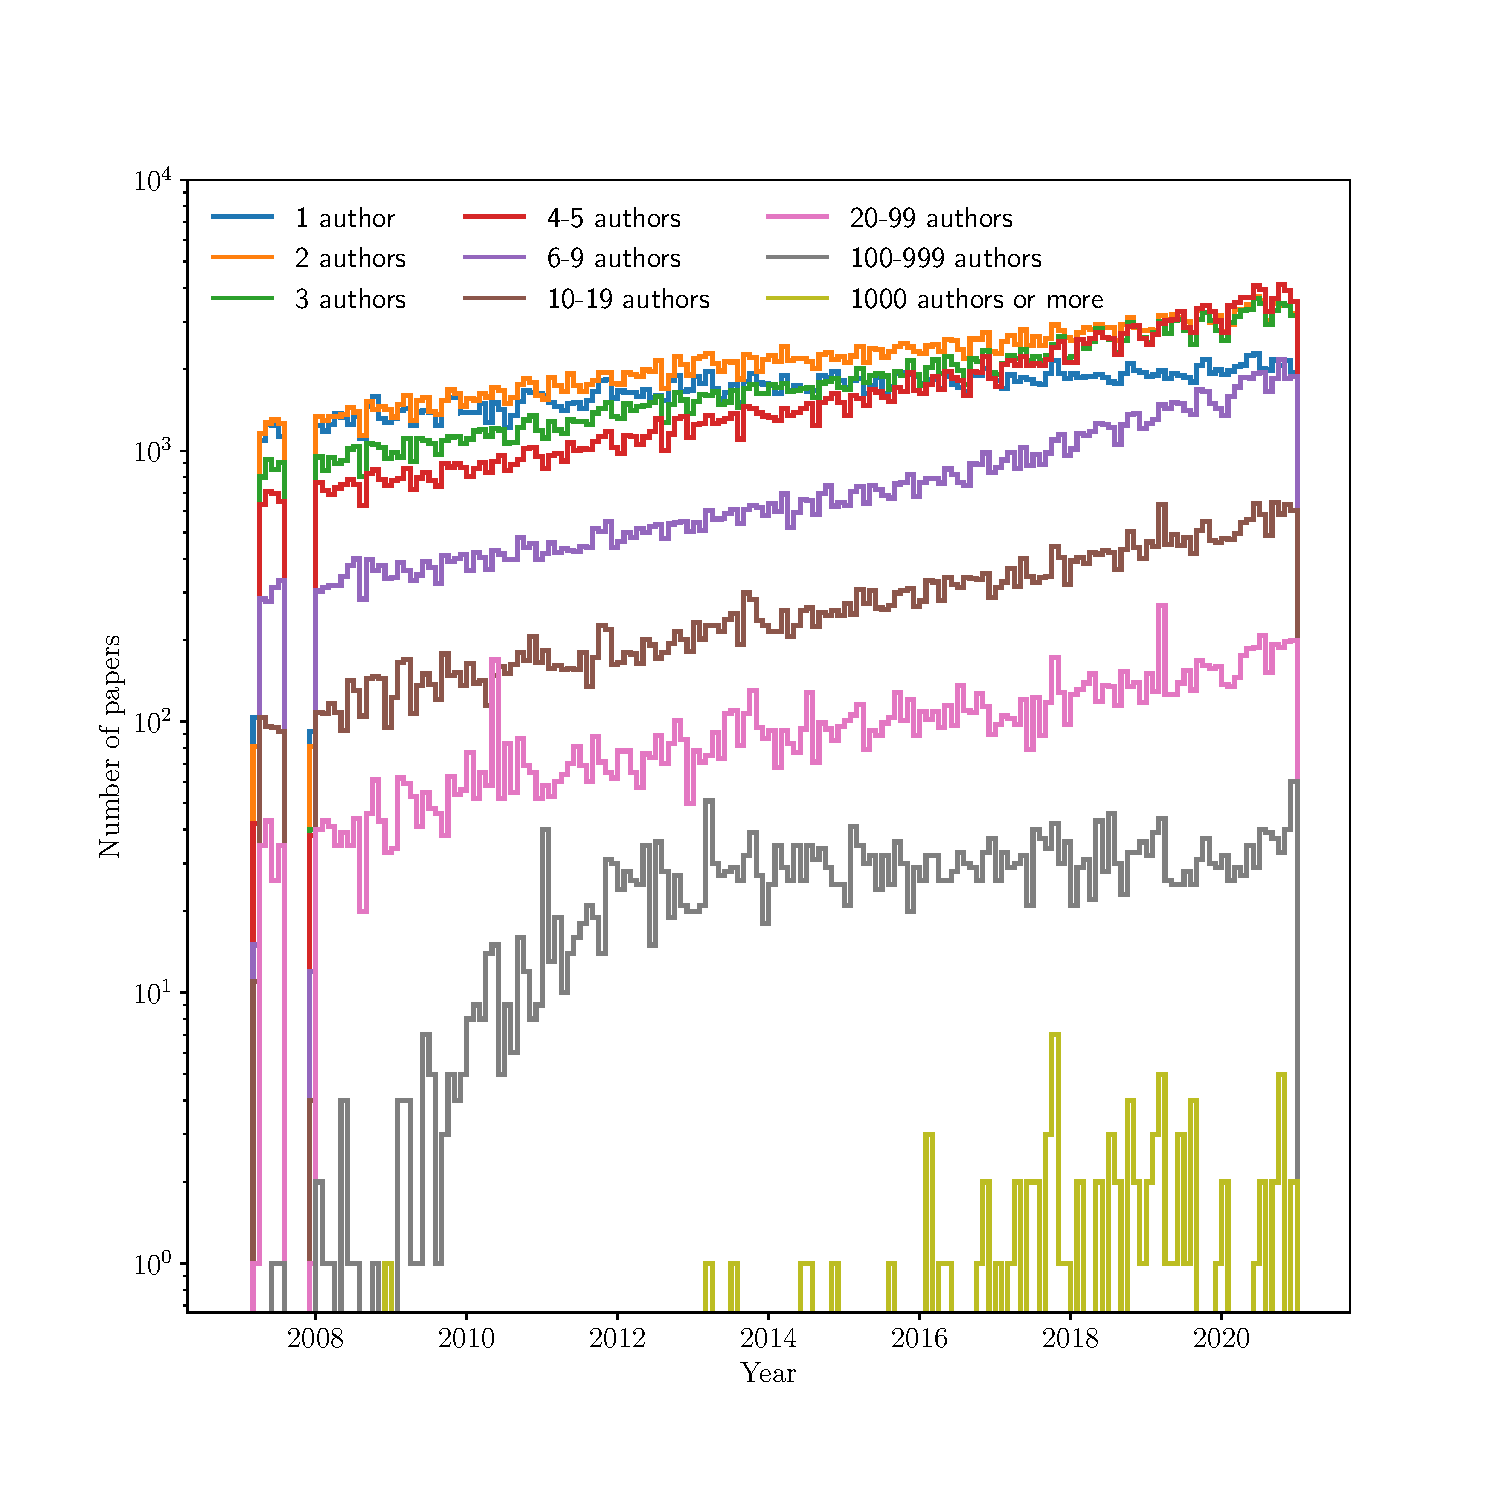
\includegraphics[width=\textwidth]{pre-prints-segmented-by-author-count}
%     \caption{Each year academics are writing more papers, with more co-authors. The typical size of the largest collaboration papers continues to increase. Single author papers are becoming rarer with time.}
%     \label{fig:pre-prints-segmented-by-author-count}
% \end{figure}


% \begin{figure}
%     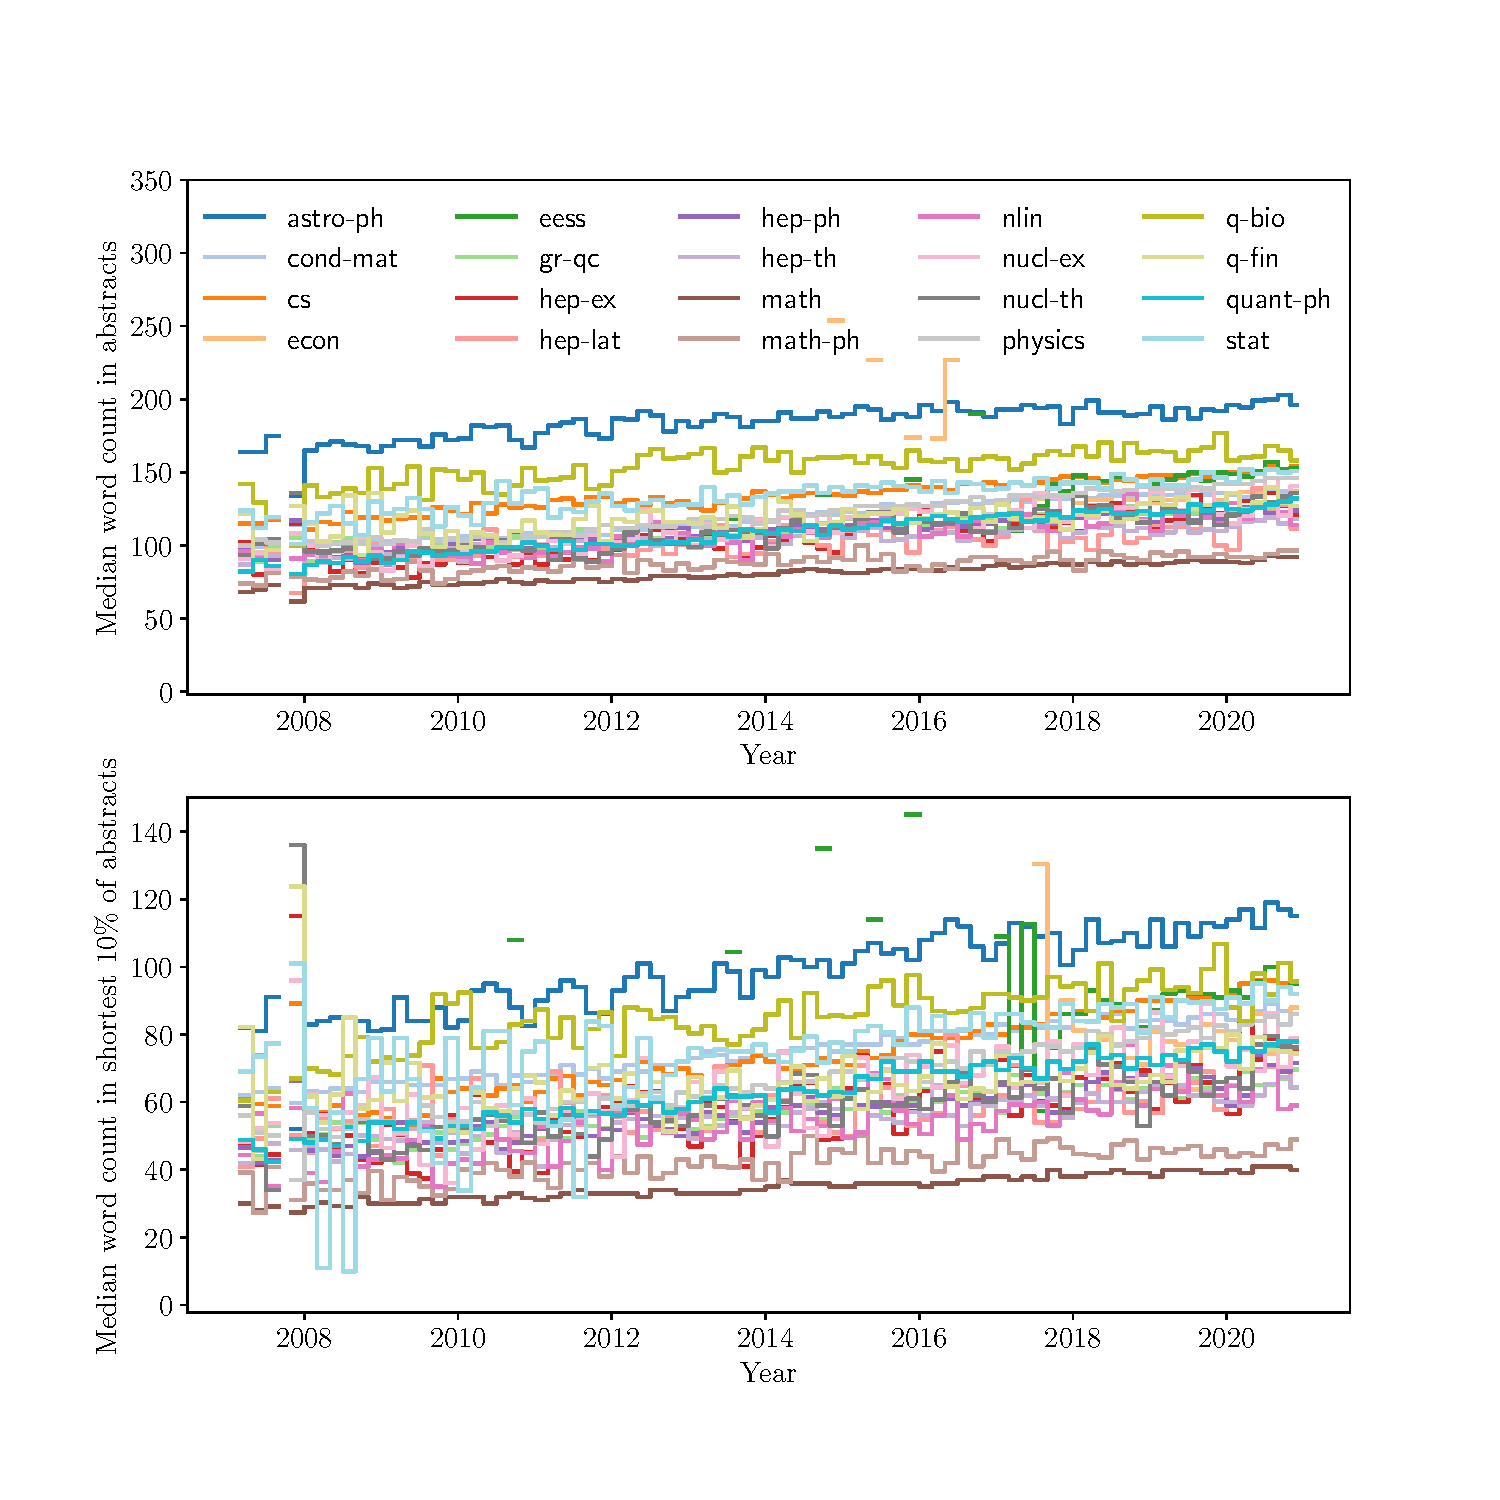
\includegraphics[width=\textwidth]{pre-prints-abstract-length}
%     \caption{The typical length of pre-print abstracts indicates that academics are writing longer papers (top). Even the shortest 10\% of abstracts in a given time bin are increasing in length (bottom).}
%     \label{fig:pre-prints-abstract-length}
% \end{figure}
 

%\begin{figure}
%	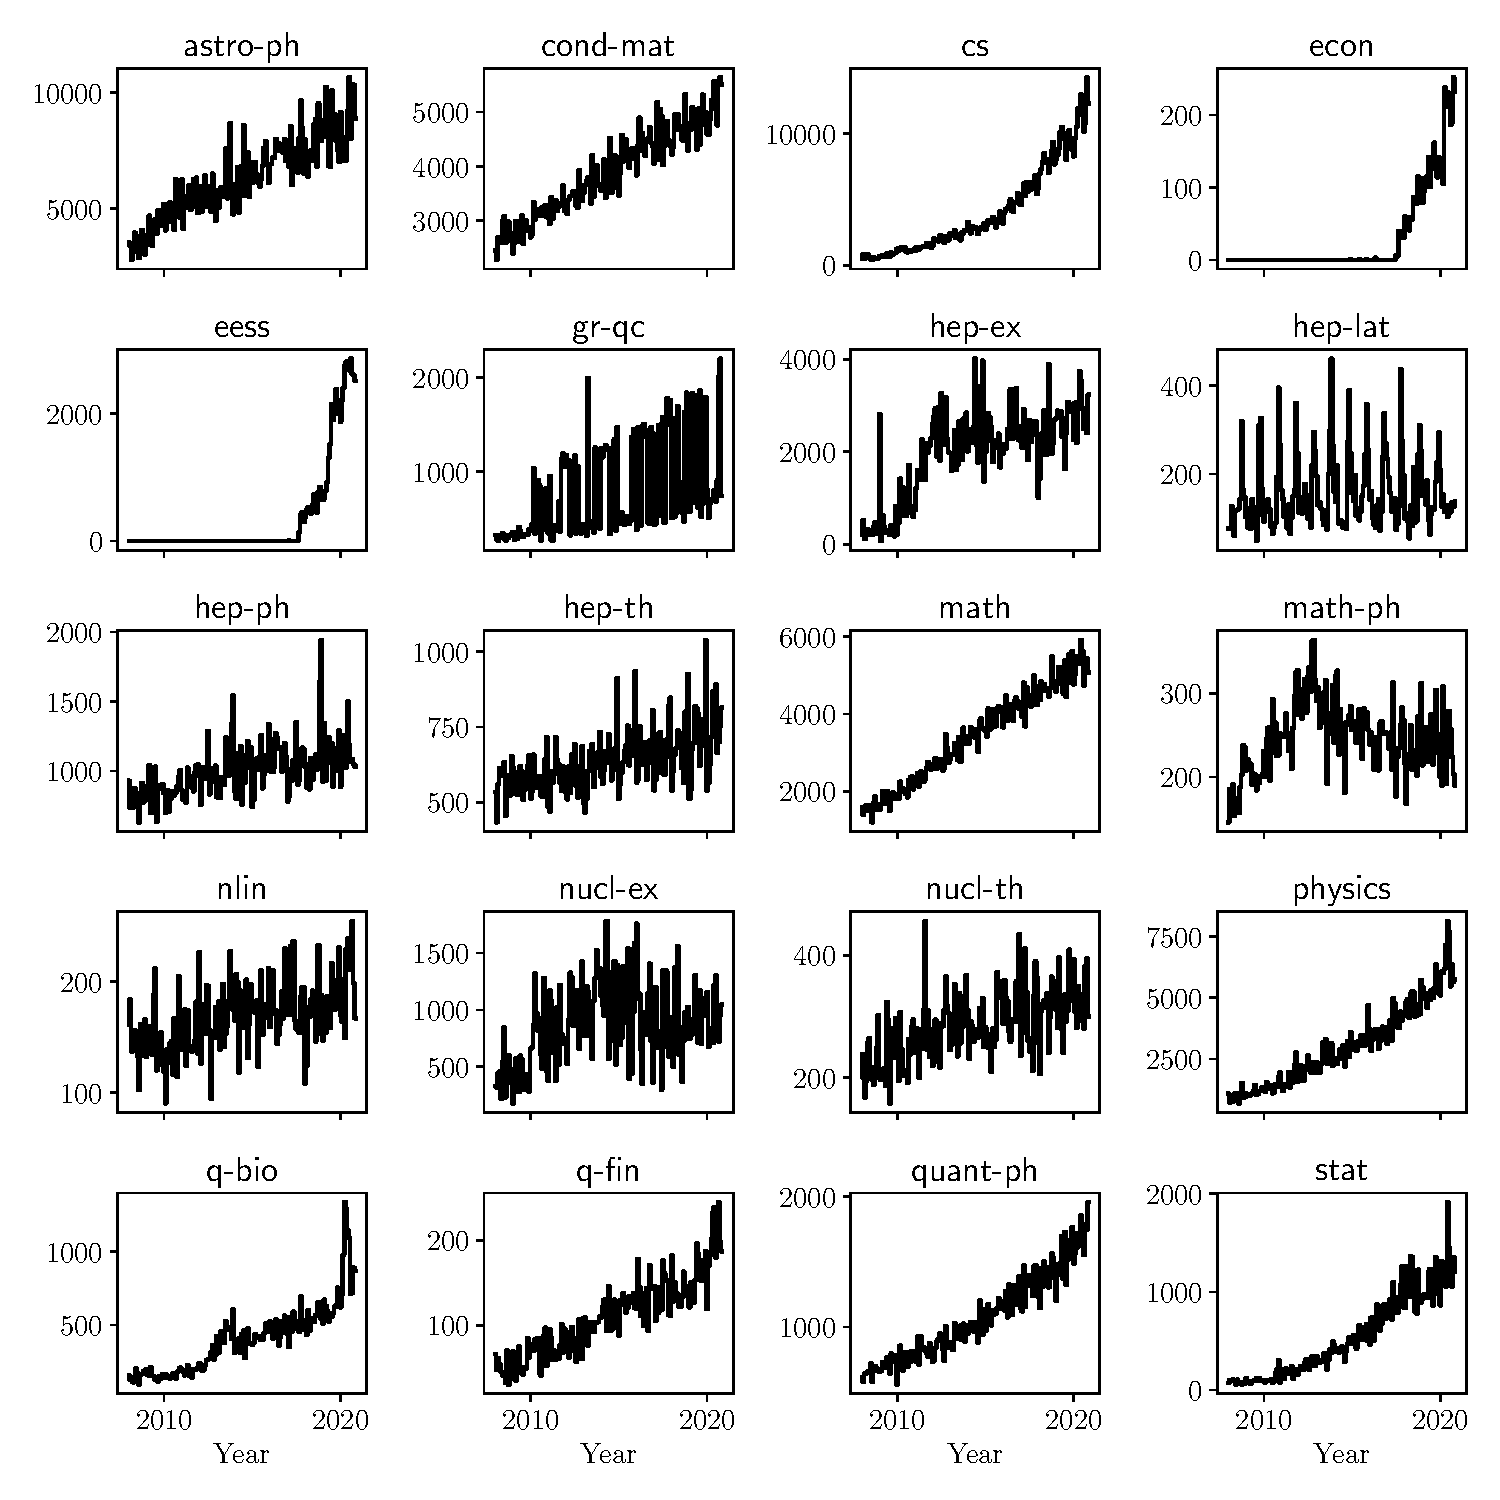
\includegraphics[width=\textwidth]{unique-authors-segmented-by-field}
%	\caption{The number of unique author names in each field as a function of time.}
%		\label{fig:unique-authors-segmented-by-field}
%\end{figure}
 




\begin{figure}
	\centering
	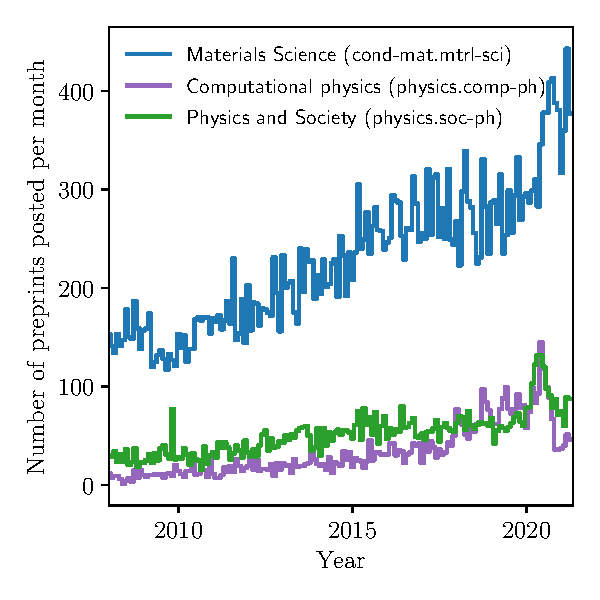
\includegraphics[width=0.5\textwidth]{winners-and-losers-of-covid}
	\caption{The number of pre-prints in selected sub-fields where the pandemic may have caused a change in publication rates.}
		\label{fig:winners-and-losers-of-covid}
\end{figure}







\section*{References}

\begin{thebibliography}{30}
%\bibitem{Iben_1967} Iben, I., Jr. Stellar Evolution. VI. Evolution from the Main Sequence to the Red-Giant Branch for Stars of Mass 1 $M_{sun}$, 1.25 $M_{sun}$, and 1.5 $M_{sun}$. \emph{Astrophys. J.} \textbf{147}, 624, doi:10.1086/149040 (1967).
\end{thebibliography}

\bibliographystyle{naturemag}


\begin{addendum}
\item[Supplementary Information] ~\\Supplementary information is linked to the online version of the paper at www.nature.com/nature.
\item[Acknowledgements] Peter Skands (Monash University) 
						and Ross Young (University of Adelaide) for comments on publication trends.

 \item[Author Information] Reprints and permissions information is
   available at www.nature.com/reprints. The authors declare that they
   have no competing financial interests. Correspondence and requests
   for materials should be addressed to andrew.casey@monash.edu
\end{addendum}

\begin{methods}

\section*{Data retrieval}

We use the \arxiv\ data set\cite{1905.00075} submitted by Cornell University to the Kaggle website. % https://www.kaggle.com/Cornell-University/arxiv
This data set includes the identifier and metadata for all pre-prints posted to \arxiv, and is updated weekly. A pre-print's identifier is defined by the year and month that the pre-print was posted, and the number of pre-prints already posted in that month (across all fields). For each pre-print the metadata includes  the title, author name(s), abstract, research field(s), and the date the pre-print was first posted. Pre-prints posted prior to 2007 use a different identifier scheme, and for this reason we have excluded pre-prints earlier than this date. The data set used for analysis includes \todo{1,379,332} pre-prints posted between \todo{2007-03-30} and \todo{2020-12-30}.



\section*{Segmenting by research field}

Pre-prints posted to the \arxiv\ can be cross-listed in multiple fields of research, and multiple sub-fields. For example, one pre-print may have a primary field of research as stellar astrophysics (astro-ph.SA) and be cross-listed in computer science. These field(s) of research are supplied by the corresponding author. It is a subjective decision whether to include more than one field of research, or what those fields of research would be. For this reason, throughout this work when we segment by research field we take the primary parent research field provided and ignore any cross-listed fields of research. When we segment pre-prints by sub-field, we similarly take the primary sub-field provided and ignore any cross-listings.

\section*{Long-term modelling of pre-print counts}

We use monthly pre-print counts per primary research field from 2007-01 until 2019-12 to make predictions for the  number of pre-prints expected in 2020. We use a Gaussian process with a quasi-periodic kernel () to model. We fix the period of the kernel to be 1 year. 



\section*{Uniquely identifying authors}

The metadata available to us does not include institutional affiliations, or identifiers that would uniquely identify an author. For these reasons, we have taken steps to minimise the effects of name confusion. There are two primary ways that name confusion could impact our inferences. In the first scenario, two people with the same name are amalgamated and treated as a single author that is on average twice as productive (or more, for very common names) as other authors. In the second scenario, an author will sometimes publish as `A.~B.~Smith', and other times publish as `A.~Smith'. A careful exploration of the data shows that this is a very frequent scenario, and if left uncorrected, would appear as many `unique' authors with half as many publications on average.

We have taken a simple approach to address name confusion. We first define a unique author by family name and the initial of the first given name (`Family-name, I.'), such that we intentionally group together authors that may share the same initial of their second given name. While our approach to name confusion is grossly simple, it is unlikely that these choices have any substantial impact on our inferences. Any common name is likely to appear in the literature early in the data set, and will not impact the conclusions we draw about how publishing changed in 2020. While common names will appear between different fields (e.g., quantitative biology and physics), by showing this as a function of time we get an intrinsic measure of the name ambiguity between fields, and we see the increase in overlap when a spike in quantitative biology papers occurs. 
Nevertheless, we manually inspected \todo{hundreds} of quantitative biology pre-prints that entirely consisted of `new authors' and cross-referenced these with Google Scholar to confirm that these authors were established researchers in other fields, and not biologists posting pre-prints for the first time.


\section*{Code availability}
The software developed to retrieve and analyse these data is publicly accessible online\footnote{https://github.com/andycasey/arxiv-covid}. All data was sourced from the \arxiv.

\end{methods}


%\section*{Additional References}
%\begin{thebibliography}{1}
%\bibitem[31]{LAMOST} Luo, A.-L. \emph{et al}. The First Data Release (DR1) of the LAMOST general survey. \emph{Res. Astron. Astrophys.} \textbf{15}, 1095, doi:10.1088/1674-4527/15/8/002 (2015).
%\end{thebibliography}



\bibliographystyle{naturemag}


\end{document}



